\documentclass[12pt,a4paper]{article}

% --- Packages ---
\usepackage[utf8]{inputenc}
\usepackage[T1]{fontenc}
\usepackage[english]{babel}
\usepackage{amsmath, amssymb, amsfonts}
\usepackage{graphicx}
\usepackage{float}
\usepackage{caption}
\usepackage{subcaption}
\usepackage{tikz}
\usepackage{pgfplots}
\pgfplotsset{compat=1.18}
\usepackage[colorlinks=true, linkcolor=blue, citecolor=blue, urlcolor=blue]{hyperref}
\usepackage{geometry}
\geometry{margin=1in}
% --- Paquetes adicionales ---
\usepackage[numbers]{natbib}  % Para usar BibTeX con numeración


% --- Title ---
\title{Research Report Title}
\author{Author Name \\
	\small Department of XYZ, University Name \\
	\small \texttt{email@example.com}}
\date{\today}

\begin{document}
	
	\maketitle
	
	\begin{abstract}
		This report presents the findings of a research study conducted on [brief topic]. The objective is to [state the goal]. The methodology includes [key methods], and the results reveal [key findings]. The implications of this study are discussed in relation to [field of application].
	\end{abstract}
	
	\tableofcontents
	\newpage
	
	% --- Sections ---
	
	\section{Introduction}
	The introduction sets the context for the research, defines the problem being investigated, and states the objectives and scope of the study. Relevant background information and previous studies are also briefly reviewed.
	
	\section{Literature Review}
	This section presents a review of relevant literature and previous work related to the research topic. It highlights gaps in existing knowledge and justifies the need for the current study.
	
	\section{Methodology}
	\subsection{Neural network design}
		\subsubsection{U-Net architecture}
		\subsubsection{U-Net-LSTM architecture}
		\subsubsection{Deep U-Net-LSTM}
	
	\subsection{Data Collection}
	Explain how the data were collected. Include instruments, tools, or datasets used.
	
	\subsection{Data Analysis}
	Describe the techniques used to analyze the data, such as statistical methods, machine learning models, or simulations.
	
	\section{Results}
	\subsection{Image Example}
	\begin{figure}[H]
		\centering
		\includegraphics[width=0.6\textwidth]{example-image.png}
		\caption{Example image illustrating the setup.}
		\label{fig:image}
	\end{figure}
	
	\subsection{Plot Example}
	\begin{figure}[H]
		\centering
		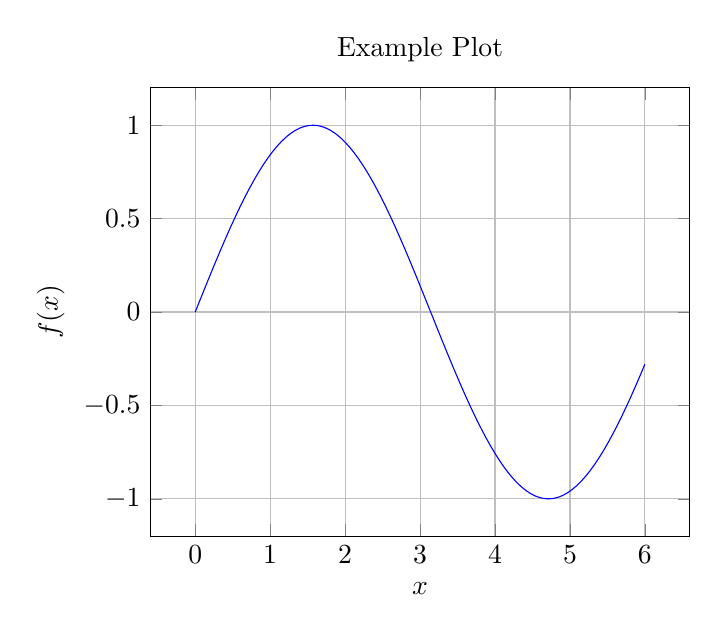
\begin{tikzpicture}
			\begin{axis}[
				title={Example Plot},
				xlabel={$x$},
				ylabel={$f(x)$},
				grid=major
				]
				\addplot[
				domain=0:6,
				samples=100,
				color=blue
				]{sin(deg(x))};
			\end{axis}
		\end{tikzpicture}
		\caption{Plot of the sine function.}
		\label{fig:plot}
	\end{figure}
	
	\section{Discussion}
	This section interprets the results presented above. Discuss their significance, compare them with expectations or previous work, and explore their implications. Highlight any limitations of the study and suggest possible reasons for unexpected findings.
	
	\section{Conclusion}
	Summarize the main findings of the research, restate the importance of the work, and suggest directions for future research.
	
	\section*{Acknowledgments}
	(Optional) Acknowledge funding sources, collaborators, or institutions that supported the research.
	
	\bibliographystyle{plain}  % O puedes usar: abbrv, alpha, ieeetr, etc.
	\bibliography{biblio}  % Nombre del archivo .bib (sin extensión)
	
\end{document}
